\section{Input-to-state stability}
\label{sec:iss}

%\begin{itemize}
%\item ISS of a particle (use an appendix if long)
%\item Parameters need for a particle to be ISS
%\item Contrast with the empirical approach of Clerc and Kennedy??
%\item Use appendix for mean and variance analysis
%\end{itemize}

In this section, we briefly review the definition of input-to-state stability (ISS) including both the conditions that guarantee it and the bound that ISS implies\cite{Jiang2001857}. 
We then show that PSO satisfies this definition when the parameters of PSO are set in the requisite range.
We also derive the bounds implied by the ISS property.
We use the ISS property to find bounds on particle motion.

Input-to-state stability analysis has been a useful tool in understanding the convergence dynamics of a system with interconnected components.
As we decompose the swarm and the particles into systems with a few component, we will apply input-to-state stability to the components to evaluate the movement of the particles.
For the position-update component, we can interpret how the bounds on $ x^{G}_{i}(k) $ and $ x^{P}_{i}(k) $ determine the positions of the particle $ x_{i}(k) $.

Before reviewing the definition of input-to-state stability, we first introduce several types of functions \cite{Jiang2001857}.
\begin{itemize}
	\item $ K $-function $ \mathbb{K} $ : a function $ \alpha  : [ 0, a ) \rightarrow [ 0, \infty ) $ is continuous, strictly increasing and $ \alpha (0) = 0 $; it is a $ K_{\infty} $-function, if $ \alpha (s) \rightarrow \infty $ as $ s \rightarrow \infty $;
	\item $ KL $-function $ \mathbb{KL} $ : a function $ \beta : [ 0, a ) \times [ 0 , \infty ) \rightarrow [ 0, \infty ) $ satisfies:
	\begin{enumerate}
		\item $ \forall t \geq 0 $, $ \beta (\cdot , t ) $ is a $ K $-function;
		\item $ \forall s \geq 0 $, $ \beta (s, \cdot) $ is decreasing and $ \beta(s,t) \rightarrow 0 $ as $ t \rightarrow \infty $.
	\end{enumerate}
	%\item Positive-definite function: a function $ \gamma (s) > 0, \forall s > 0 $ and $ \gamma (0) = 0 $.
\end{itemize}

These functions are used to define input-to-state stability in Definition \ref{def:iss}.

\begin{mydef}[Input-to-state stable \cite{Jiang2001857}]
\label{def:iss}

For $ x $, a discrete-time system defined as follows:
\begin{equation}
\label{eq:dis_nonlinear}
x(k+1) = f( x(k) , u(k) ),
\end{equation}
with $ f(0,0) = 0 $
\footnote{This means that $ x = 0 $ is an equilibrium of the 0-input system.}, the system is \emph{(globally) input-to-state stable} if there exist a $ KL $-function $ \beta  $ and a $ K $-function $ \gamma $ such that, for each input $ u \in l^{m}_{\infty} $ and each $ \xi \in \mathbb{R}^{n} $, it holds that $  \forall k \in \mathbb{Z}^{+} $,
\begin{equation}
\label{eq:def_iss}
| x(k, \xi, u) | \leq \beta (| \xi |, k) + \gamma (\lVert u \rVert).
\end{equation}
\end{mydef}

The $ \beta () $ term in equation \eqref{eq:def_iss} defines an initial bound with a decaying property.
The $ \gamma () $ term in equation \eqref{eq:def_iss} defines a bound determined by the input.
This means that the influence $ \beta () $ term gradually decreases to zero and the position is bounded by a range determined by the bound on the input.


The input-to-state stability analysis also provides the tool for the analysis of the convergence of PSO and the analysis of bounds on particle motion.
PSO is designed to strike an effective balance between \emph{exploring} and \emph{exploiting} a fitness landscape.
A bound on a particle's state is an indicator of the nature of that balance.
When this bound is large the particle is exploring.
However, as a particle finishes exploring and reach stagnation, a particle's position should converge.

Input-to-state stability implies that the state of the system is bounded in a range determined by the bounds on the input.
Before stagnation, when the personal best and global best values have not converged, we can expect only a loose bound on the particle state.
These looser bounds reflect both what is know about the what is know about the update process itself and what is know about the inputs to the update process, that is, the personal best and the global best.

We call the bounds on the global best and personal best the ``exploit radius'' and the bounds on the particle's position a ``explore radius''.
The ratio of the explore radius to the exploit radius is determined by the parameters of the position-update component.
However, if the personal best and global best converge to an estimated optimal position, the exploit radius falls to zero and the explore radius converges to a bound.

\begin{figure}
\centering
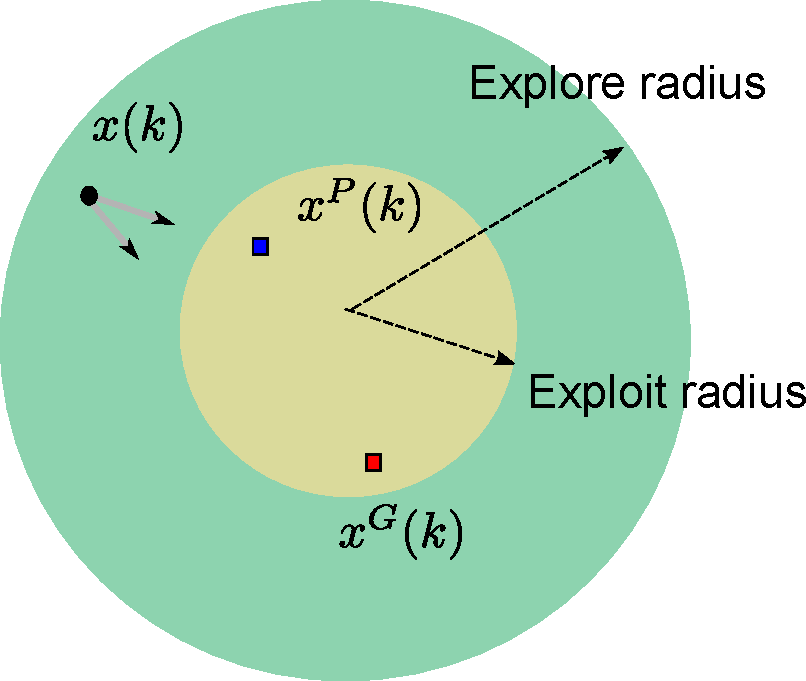
\includegraphics[width=0.5\linewidth]{./fig/explore_and_exploit.pdf}
\caption{Exploration and exploitation.}
\label{fig:explore_and_exploit}
\end{figure}

In the case of PSO and as shown in Figure \ref{fig:sys_flow}, if each component (representing a single dimension) is input-to-state stable, the position-update component which combines all the dimensions is also input-to-state stable.
Thus we have property \ref{prop:iss:parallel}.
\begin{myprop}
\label{prop:iss:parallel}
The position-update component is input-to-state stable if the update in each dimension is input-to-state stable.
\end{myprop}
This simplifies the analysis of the system since it allows us to consider each dimension separately.
In our analysis of the PSO algorithm, we seek to understand how the particles converge to some position $ x^{R} $, which is intended (not guaranteed) by the algorithm to be the optimal position.
For this analysis we use a one-dimension particle and extract the linear form of the position-update component.
As noted above, the one dimensional case can be extended to many dimensions.

%\subsection{Input-to-state stability of the position update}

%An ISS-Lyapunov function, defined above, can be used to prove the input-to-state stability of a system and analyze the state bound\cite{Jiang2001857}.
%We will use the ISS-Lyapunov-function approach in the proof given later in this section.

\subsection{Conditions for input-to-state stability for position update in PSO}
\label{sec:iss_conditions}

Using the definition of the PSO position update as given in \eqref{eq:pso_up_linalg_simp}, PSO can be shown to be ISS as defined in definition \ref{def:iss}.

\begin{mythm}
\label{thm:iss}
The system \eqref{eq:pso_up_linalg_simp} is input-to-state stable, when $ | \lambda_{\max} ( A(k) ) | < 1 $.
\begin{proof}
The proof follows the ISS-Lyapunov-function approach. 
The ISS-Lyapunov function, defined in Appendix \ref{sec:iss_lyapunov:func}, can be used to prove the input-to-state stability of a system and analyze the state bound\cite{Jiang2001857}.
The details of the proof are given in Appendix \ref{sec:thm:iss:proof}.
\end{proof}
\end{mythm}

Note that in equation \eqref{eq:pso_up_linalg_simp},
$ [ v(k), x(k) - x^{*} ]^{T} = [0, 0]^{T} $ is an equilibrium position when the input $ [ x^{G}(k) - x^{*} , x^{P}(k) - x^{*} ]^{T} = [0, 0]^{T} $.
Without loss of generality, for an arbitrary optimization problem $ x^{*} $ would typically not be at the origin. 
In such a problem, input-to-state stability means that the boundaries of $ | v(k) | $ and $ | x(k) - x^{*} | $ would be transformed and thus determined by $ | x^{G}(k) - x^{*} | $ and $ | x^{P}(k) - x^{*} | $,
but the properties of ISS apply independent of where the function is centered.
Having shown that PSO is ISS we can now state a bound on particle position.

\begin{mythm}
\label{thm:state_bound}
Given the bound on the input $ \lVert u \rVert $ in the position update component, we have the bound on the particle position from \eqref{eq:pso_up_linalg_simp}.
\begin{equation}
\label{eq:state_bound}
\forall k, 
| x(k+1) - x^{R} | \leq \max ( | x(0) - x^{R} | , \gamma ( | [ x^{G}(k) - x^{R}, x^{P}(k) - x^{R} ]^{T} | ) ),
\end{equation}
in which $ \gamma = \alpha_{3}^{-1} \circ \sigma $.
($ \alpha_{3} $ and $ \sigma $ are defined in Appendix \ref{sec:thm:iss:proof}.)
The $ \max $ part is needed to account for the effect of the starting point, represented by the first parameter. Eventually the effect of the starting point no longer affects the system, formally:
\begin{equation}
\label{eq:state_bound:conv}
\exists T, \forall k \geq T, 
|  x(k+1) - x^{R} | \leq \gamma ( | [ x^{G}(k) - x^{R}, x^{P}(k) - x^{R} ]^{T} | ).
\end{equation}
\begin{proof}
The proof is given in Appendix \ref{sec:thm:state_bound:proof}.
\end{proof}
\end{mythm}

Figure \ref{fig:boundary} gives an example on how a particle's boundary is determined by the personal best and global best.

\begin{figure}
\centering
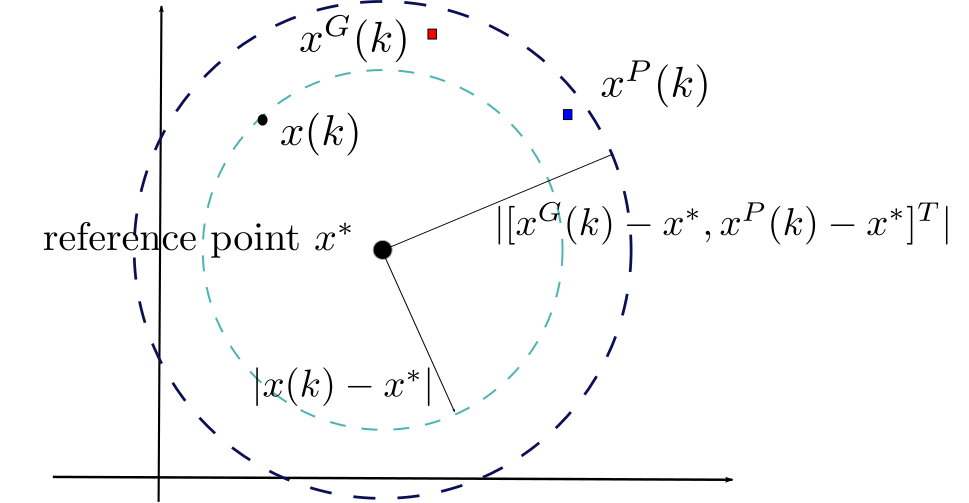
\includegraphics[width=0.7\linewidth]{./fig/boundary}
\caption{A bound on a particle's position by a reference point $ x^{*} $ from Equation \ref{eq:state_bound:conv}.
The ratio of wo radii indicates $ \gamma $.}
\label{fig:boundary}
\end{figure}

\begin{mycoro}
\label{coro:param_unit_disc}
Write $ A(k) = 
\begin{bmatrix}
\chi & - \chi \phi \\
\chi & 1 - \chi \phi
\end{bmatrix}
$, in which
$ \phi \in [0,  \phi^{P} + \phi^{G} ] $ and $ \chi \in ( 0, 1 ) $.
When $ \phi \in (0 , \frac{2(1+\chi)}{\chi} ) $, the system \eqref{eq:pso_up_linalg_simp} is input-to-state stable.
\begin{proof}
The proof is given in Appendix \ref{sec:coro:param_unit_disc:proof}.
\end{proof}
\end{mycoro}

Figure \ref{fig:paramSpace} shows the parameter space.
The x-axis is $ \phi = \phi^{P} + \phi^{G} $ and the y-axis is $ \chi $.
The stable region in red is obtained from eigenvalue test on Theorem \ref{thm:iss} and the yellow boundary is obtained from Corollary \ref{coro:param_unit_disc}.
\begin{figure}
\centering
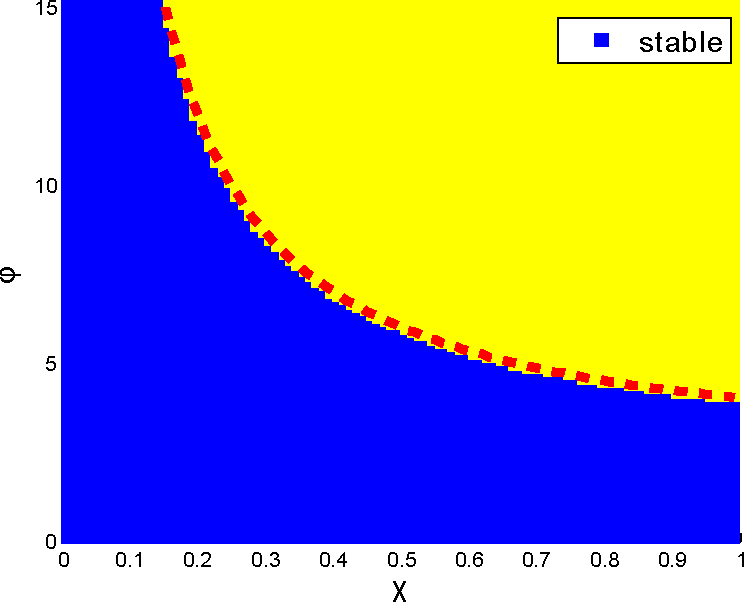
\includegraphics[width=0.5\linewidth]{./fig/param2}
\caption{Parameter space}
\label{fig:paramSpace}
\end{figure}

\subsection{Moment Analysis}
\label{sec:moment_analysis}

Using the same perspective of the feedback cascade system, the input-to-stable stability analysis can also be applied to moment analysis.
Like the others \cite{Jiang20078,Poli:2008:DSS:1384929.1384944}, we derive models for the statistical features (moments) of the particle's position at stagnation.
In contrast to this prior work,
input-to-state stability analysis can also provide bounds before a particle reaches stagnation.

We adopt the approach of Jiang, Luo \& Yang \cite{Jiang20078} to construct an ISS model for the mean.
Using that model $ E( x(k) ) $ converges to 
\begin{equation}
\nonumber
\hat{x} = \frac{\phi^{P} x^{P} + \phi^{G} x^{G} }{ \phi^{P} + \phi^{G} } 
\end{equation}
in stagnation.
If we treat $ \hat{x} $ as a swarm average estimation on the optimum, we are interested in how $ E( x(k) ) $ deviates from $ \hat{x} $.
\begin{equation}
\label{eq:pso1_alg_mean_linalg:final}
\begin{aligned}
\begin{bmatrix}
E( x(k+1) ) - \hat{x} \\
E( x(k) ) - \hat{x}
\end{bmatrix}
& = 
A_{m}
\begin{bmatrix}
E( x(k) ) - \hat{x} \\
E( x(k-1) ) - \hat{x}
\end{bmatrix}
\\ & +
B_{m}
\begin{bmatrix}
E( x^{P}(k) ) - \hat{x}\\
E( x^{G}(k) ) - \hat{x}
\end{bmatrix},
\end{aligned}
\end{equation}
with 
\begin{equation}
\nonumber
A_{m} = \begin{bmatrix}
1 + \chi - \frac{ \chi \phi^{P} }{2} - \frac{ \chi \phi^{G} }{2} & -\chi \\
1 & 0
\end{bmatrix}
\end{equation}
and
\begin{equation}
\nonumber
B_{m} = \begin{bmatrix}
\frac{ \chi \phi^{P} }{2} & \frac{ \chi \phi^{G} }{2} \\
0 & 0
\end{bmatrix}.
\end{equation}

The convergence of $ E( x(k) ) $ in stagnation is given in \cite{Jiang20078,Poli:2008:DSS:1384929.1384944}.
Even without the stagnation assumption, 
the input-to-state stable analysis on equation \eqref{eq:pso1_alg_mean_linalg:final} indicates how $ E(x(k)) $ will deviate from $ \hat{x} $ anytime we know how $ E( x^{G}(k) ) $ and $ E( x^{P}(k) ) $ deviate from $ \hat{x} $. Stagnation is a simple case of knowing how $ E( x^{G}(k) ) $ and $ E( x^{P}(k) ) $ deviate from $ \hat{x} $. This special case is discussed more later in this paper.

We now proceed to show the conditions that must hold for the mean model to be ISS.
\begin{mythm}
\label{thm:iss:mean}
	The system \eqref{eq:pso1_alg_mean_linalg:final} is input-to-state stable, if $ | \lambda_{\max} ( A_{m} ) | < 1 $.
	\begin{proof}
		The proof process is similar with Theorem \ref{thm:iss}, but we can get a constant symmetric positive definite $ Q_{m} $ from $ A_{m}^{T} P A_{m} - P = - Q_{m} $.
	\end{proof}
\end{mythm}

%\begin{mycoro}
%When $ | \lambda_{\max} ( A_{m} ) | < 1 $, the system %\eqref{eq:pso1_alg_mean_linalg:final} is %input-to-state stable.
%\end{mycoro}

Similar to Corollary \ref{coro:param_unit_disc}, we have Corollary \ref{coro:param_unit_disc:mean} for parameter selection on mean convergence.
Note that when the condition in Corollary \ref{coro:param_unit_disc} is satisfied, the condition in Corollary \ref{coro:param_unit_disc:mean} is also guaranteed.
This means that when the system \eqref{eq:pso_up_linalg_simp} is input-to-state stable, the mean dynamics \eqref{eq:pso1_alg_mean_linalg:final} is also input-to-state stable.

\begin{mycoro}
\label{coro:param_unit_disc:mean}
Write $ A_{m} = \begin{bmatrix}
1 + \chi - \frac{ \chi \phi^{P} }{2} - \frac{ \chi \phi^{G} }{2} & -\chi \\
1 & 0
\end{bmatrix} 
$, in which
$ \phi \in [0,  \phi^{P} + \phi^{G} ] $ and $ \chi \in ( 0, 1 ) $.
When $ \phi \in \left( 0 , \frac{4(1+\chi)}{\chi} \right) $, the system \eqref{eq:pso1_alg_mean_linalg:final} is input-to-state stable.
\begin{proof}
The proof is given in Appendix \ref{sec:coro:param_unit_disc:proof:mean}.
\end{proof}
\end{mycoro}


Similar to Theorem \ref{thm:state_bound}, we can use the $ Q_{m} $ to determine the state bound.
\begin{mycoro}
\label{coro:bound:mean}
If the system \eqref{eq:pso1_alg_mean_linalg:final} is input-to-state stable, we have a bound 
\begin{equation}
\begin{aligned}
\exists & T , \forall  k > T, \\
& | E( x(k) ) - \hat{x} | \leq  \gamma_{m} | [ E( x^{P}(k) ) - \hat{x} ,  E( x^{G}(k) ) - \hat{x} ]^{T} |,
\end{aligned}
\end{equation}
with 
\begin{equation}
\gamma_{m} = \frac{ 2 \lVert A_{m} \rVert^{2} \lVert B_{m} \rVert^{2} + \lambda_{min}( Q_{m} )^{2} \lVert B_{m} \rVert^{2} }{ 2( \lambda_{min}( Q_{m} ) )^{3} }.
\end{equation}
\end{mycoro}

In a similar way, we can apply the input-to-state stability analysis to the variance model \cite{Jiang20078} and higher order moment models \cite{Poli:2007:EAS:1276958.1276977}.

%Answer two questions here
% a) why we need iss of position update 
% b) what else do we need for iss

Since by Theorem \ref{thm:iss} PSO is ISS, and therefore by Theorem \ref{thm:state_bound} the stability of the cascade system depends on the output of the input-update component. 
We can say:
\begin{enumerate}
\item If the input-update component generates converging personal best and global best, the bound of the particle position will converge;
\item If the personal best and global best vary within a bound, the particle will converge within a bound;
\item If the personal best and global best become constant, the particle will converge within a bound.
\item If the personal best and global best are constant and the same, the particle will converge toward the global best.
\end{enumerate}
By Theorem \ref{thm:iss:mean} and \ref{coro:bound:mean}, we can make similar statements about the particle mean.
As well, this boundary analysis could be applied to higher moments.

Furthermore, by equation \eqref{eq:state_bound}, we know that the convergence of a particle's position $ x(k) $ to $ x^{*} $ depends on how $ x^{P}(k) $ and $ x^{G}(k) $ converge to $ x^{*} $ when the position-update component is input-to-state stable.
In particular, the bound on the distance between a particle's position and  $ x^{*} $ is determined by the initial distance $ x(0) -  x^{*} $, $ x^{P}(k) -  x^{*} $ and $ x^{G}(k) -  x^{*} $.

The input-to-state stability of the position update component makes the movement of a particle bounded in a range that covers the global best and the personal best.
This property provides the chance that the particle exploits the regions near around the personal best and the global best.
We can have:
\begin{enumerate}
\item If the personal best and global best converge, the bound of the particle position will converge;
\item If the personal best and global best vary within a bound, the particle will converge within a bound;
\item If the personal best and global best become constant, the particle will converge to a point.
\end{enumerate}
Furthermore, by \eqref{eq:state_bound}, we know that the convergence of a particle's position $ x(k) $ to $ x^{R} $ depends on how $ x^{P}(k) $ and $ x^{G}(k) $ converge to $ x^{R} $, if the position update component is input-to-state stable.
In particular, the boundary of the distance between a particle's position and  $ x^{R} $ is determined by the initial distance $ x(0) -  x^{R} $, $ x^{P}(k) -  x^{R} $ and $ x^{G}(k) -  x^{R} $.

When the position update component is input-to-state stable, the input-to-state stability of the particle is determined by the input-to-state stability of the personal best update component.
However, the input-to-state stability of the input update component depends on the fitness distribution, which could not be guaranteed in many cases.
In section \ref{sec:particle}, we will analyze the behavior of the particle when the position update component is input-to-state stable.
We will later extend the analysis to the swarm in section \ref{sec:swarm}.

